\documentclass[unicode,11pt,a4paper,oneside,numbers=endperiod,openany]{scrartcl}

\usepackage{assignment}
\usepackage{textcomp}
\usepackage{amssymb}
\usepackage{mathtools}
\usepackage{subcaption}
\usepackage{float}

\begin{document}

\graphicspath{{./img/}}

\setassignment
\setduedate{3 December 2019, 23:55}

\serieheader{High Performance Computing}{2019}{Student: Gabriel Fernandes de Oliveira}{Discussed with: N/A}{Solution for Assignment 6}{}
\newline

\section*{Adding MPI to the mini-app}

\section{Initialize and finalize MPI \punkte{5}}

The initialization of the MPI and the variables $mpi\_rank$ and $mpi\_size$ were done in the beginning of the main function in \textit{main.cpp}.

\begin{figure}[H]
    \centering
    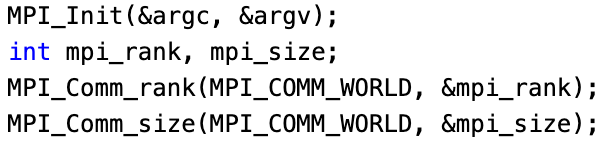
\includegraphics[width=.5\linewidth]{initialize}
\end{figure}

Whereas the finalization of the MPI was inserted right before the \textit{return 0;} of the main function.

\begin{figure}[H]
    \centering
    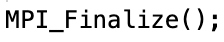
\includegraphics[width=.3\linewidth]{finalize}
\end{figure}

\section{Create a Cartesian topology \punkte{10}}


\section{Change linear algebra functions \punkte{5}}

\section{Exchange ghost cells \punkte{60}}

\section{Testing \punkte{20}}


\end{document}
